\documentclass{book}

\usepackage[spanish]{babel}


\usepackage[letterpaper,top=2cm,bottom=2cm,left=3cm,right=3cm,marginparwidth=1.75cm]{geometry}

\usepackage{amsmath}
\usepackage{graphicx}
\usepackage[colorlinks=true, allcolors=blue]{hyperref}


\title{Accidentes de Tráfico en Nueva Zelanda}
\author{Paola Espinoza Hernández, C32715 \and Jeikel Navarro Solís, C25518 \and Gabriel Sanabria Alvarado, C27184}

\begin{document}
\maketitle

\chapter*{Bitácora 1}

\section{Planificación}

\subsection{Pregunta de investigación}
¿Cuáles variables tienen mayor impacto en la severidad de los accidentes de tráfico en Nueva Zelanda?

\subsubsection{Definición de la idea}

La idea principal se centra en la identificación y análisis de los factores que influyen en la gravedad de los accidentes de tráfico en Nueva Zelanda. 

\subsubsection{Conceptualización de la idea}

Los accidentes de tráfico se refieren a aquellos accidentes ocurridos sobre la vía, determinados por condiciones y actos irresponsables potencialmente previsibles, atribuidos a factores humanos, vehículos preponderantemente automotores, condiciones climatológicas, señalización y caminos, los cuales ocasionan pérdidas prematuras de vidas humanas y/o lesiones, así como secuelas físicas o psicológicas, perjuicios materiales y daños a terceros.

La severidad de los accidentes de tráfico se refiere al grado de daño o consecuencias que resultan de un siniestro vial, pudiendo clasificarse en leves, graves o fatales. Diversos factores pueden influir en esta severidad, entre los que se incluyen elementos ambientales, vehiculares, humanos y de infraestructura.

Si bien esta investigación se centra en identificar las variables con mayor impacto en la severidad de los accidentes de tráfico de Nueva Zelanda, el enfoque puede extenderse para incluir análisis comparativos con otros países, evaluar la efectividad de políticas de seguridad vial o desarrollar modelos predictivos de riesgo. Esto permite abordar distintos métodos y perspectivas dentro del tema, volviendo el estudio mucho más profundo para futuras investigaciones.

Este estudio busca proporcionar cierta evidencia empírica para una correcta elaboración de las estrategias de seguridad vial en Nueva Zelanda. Al identificar los factores que impactan principalmente en la severidad de los accidentes, se pueden diseñar políticas públicas más efectivas y medidas preventivas que reduzcan la mortalidad y el impacto socioeconómico de estos incidentes.

\subsubsection{Identificación de tensiones}

Las tensiones que afectan la severidad de los accidentes surgen de la interacción compleja de diferentes variables, lo que complica la predicción y análisis de los accidentes. Por ejemplo, las condiciones meteorológicas adversas, como la lluvia o la niebla, pueden disminuir la visibilidad y así provocar un aumento en la probabilidad de accidentes graves, pero esto se ve intensificado por la falta de señales de tráfico adecuadas o un control de tráfico deficiente, lo que genera que ocurran accidentes más severos. A su vez, las zonas con límites de velocidad más altos o una velocidad recomendada no respetada en ciertas áreas, como zonas cercanas a peatones o zonas con pendientes pronunciadas, también contribuyen a un aumento en la severidad de los accidentes.

Las condiciones de las calles como superficies mojadas, resbaladizas o mal mantenidas pueden influir significativamente en la severidad del accidente, aumentando la cantidad de lesiones graves o incluso de muertes. Por otro lado, los días festivos pueden llegar a ser un problema a considerar, pues estos suelen incrementar el tráfico en las carreteras, que aumenta a su vez el riesgo de fuertes accidentes. 

Por otro lado, la presencia de peatones en las zonas de tráfico aumenta el riesgo de accidentes graves, ya que, incluso a velocidades moderadas, el impacto con un peatón puede ser fatal. Este conflicto se intensifica si las zonas peatonales no están bien señalizadas o si los conductores no prestan suficiente atención.

Un punto importante a considerar es el caso de las vías que se encuentran en zonas montañosas, donde las pendientes y la mala calidad del asfalto pueden hacer que los vehículos pierdan el control, y como consecuencia, ocurran accidentes graves. Las condiciones climáticas como la lluvia pueden agravar este riesgo, lo que genera una mayor severidad en los accidentes en estas zonas. Por último, los accidentes en áreas rurales suelen ser más graves no por la naturaleza del accidente en sí, sino por la falta de accesibilidad rápida a los servicios de emergencia, por lo que la respuesta a los accidente es más lenta, de modo que aumenta la probabilidad de lesiones graves o muertes.

\subsubsection{Reformulación de la idea en modo de pregunta}

\begin{enumerate}
    \item ¿Qué variables tienen la mayor influencia en la severidad de los accidentes de tráfico en Nueva Zelanda?
    \item ¿Cómo afectan factores como el clima, el límite de velocidad y las condiciones de la carretera a la gravedad de los accidentes de tráfico en Nueva Zelanda?
    \item ¿Existen patrones entre la presencia de peatones, el tipo de control de tráfico y la gravedad de los accidentes en Nueva Zelanda?
    \item ¿Por qué es importante identificar las variables que influyen en la severidad de los accidentes de tráfico en Nueva Zelanda?
\end{enumerate}

\subsubsection{Argumentación de la pregunta}

\subsubsection{Pregunta 1: ¿Qué variables tienen la mayor influencia en la severidad de los accidentes de tráfico en Nueva Zelanda?}

\textbf{Contraargumentos}
\begin{itemize}
    \item \textbf{Lógica:} ALgunas de las variables puede que estén interconectadas, haciendo más díficil clasificar el impacto directo de cada una de ellas.
    \item \textbf{Ética:} La recopilación de datos puede estar incompleta o incluso sesgada, llegando a afectar los resultados y su validez.
    \item \textbf{Emocional:} Algunas variables podrían llegar a considerarse para la población en general, disminuyendo el interés en la investigación.
\end{itemize}

\textbf{Argumentos}
\begin{itemize}
    \item \textbf{Lógica:} Utilizando modelos estadísticos y aprendizaje automático, se pueden identificar correlaciones significativas entre las variables y la severidad del accidente.
    \item \textbf{Ética:} Se dará uso de fuentes oficiales y métodos rigurosos para garantizar la veracidad de los datos.
    \item \textbf{Emocional:} Comprender los factores más influyentes permitirá implementar medidas preventivas, reduciendo lesiones y muertes.
\end{itemize}

\textbf{Conclusión:} La identificación de variables clave ayudará a diseñar mejores estrategias de seguridad vial. ¿Cómo se pueden optimizar los recursos para maximizar la reducción de accidentes?

\subsubsection{Pregunta 2: ¿Cómo afectan factores como el clima, el límite de velocidad y las condiciones de la carretera a la gravedad de los accidentes de tráfico en Nueva Zelanda?}

\textbf{Contraargumentos}
\begin{itemize}
    \item \textbf{Lógica:} La relación entre estas variables y la severidad del accidente no siempre es directa, ya que otros factores pueden influir.
    \item \textbf{Ética:} La recopilación de datos sobre condiciones climáticas y su correlación con accidentes puede verse afectada por la falta de registros precisos.
    \item \textbf{Emocional:} Algunas personas pueden minimizar el impacto del clima o del estado de las carreteras en los accidentes, atribuyéndolos exclusivamente a la imprudencia.
\end{itemize}

\textbf{Argumentos}
\begin{itemize}
    \item \textbf{Lógica:} Las condiciones climáticas adversas pueden llegar a aumentar el riesgo de accidentes.
    \item \textbf{Ética:} El uso de datos meteorológicos y registros viales confiables permitirá una evaluación objetiva.
    \item \textbf{Emocional:} Crear conciencia sobre estos factores puede incentivar a la creación de políticas enfocadas en la mejora de la infraestructura vial y alertar a los conductores.
\end{itemize}

\textbf{Conclusión:} Analizar estos factores dar inicio a la implementación de políticas de seguridad más adecuadas. ¿Cómo se pueden mejorar las alertas para conductores en condiciones peligrosas?

\subsubsection{Pregunta 3: ¿Existen patrones entre la presencia de peatones, el tipo de control de tráfico y la gravedad de los accidentes en Nueva Zelanda?}

\textbf{Contraargumentos}
\begin{itemize}
    \item \textbf{Lógica:} La relación entre peatones y accidentes puede depender de factores aleatorios como el comportamiento humano.
    \item \textbf{Ética:} Determinar la responsabilidad en los accidentes que involucran peatones puede ser subjetivo.
    \item \textbf{Emocional:} La percepción de seguridad vial varía entre peatones y conductores puede generar conflictos de intereses.
\end{itemize}

\textbf{Argumentos}
\begin{itemize}
    \item \textbf{Lógica:} Los datos pueden revelar patrones en zonas con alta incidencia de atropellos, permitiendo estrategias de mitigación, esto acompañado de estimaciones generadas mediante argumentos estadísticos.
    \item \textbf{Ética:} La transparencia en el análisis de datos garantizará recomendaciones imparciales.
    \item \textbf{Emocional:} Mejorar la seguridad de peatones puede reducir muertes y fomentar un transporte urbano más seguro.
\end{itemize}

\textbf{Conclusión:} Analizar estos patrones contribuirá a aminorar los choques hacia peatones y mejorar la convivencia vial. ¿Qué medidas pueden tomarse para garantizar la seguridad de peatones en zonas de alto tráfico?

\subsubsection{Pregunta 4: ¿Por qué es importante identificar las variables que influyen en la severidad de los accidentes de tráfico en Nueva Zelanda?}

\textbf{Contraargumentos}
\begin{itemize}
    \item \textbf{Lógica:} Se podría pensar que, en lugar de investigar las variables, se deberían tomar medidas generales de seguridad vial sin tomar en cuenta un análisis tan detallado.
    \item \textbf{Ética:} Algunos pueden cuestionar la priorización de ciertos factores sobre otros en la investigación.
    \item \textbf{Emocional:} Las personas pueden no percibir el impacto de estos estudios hasta que enfrentan una situación de riesgo.
\end{itemize}

\textbf{Argumentos}
\begin{itemize}
    \item \textbf{Lógica:} Conocer las variables más influyentes permitirá diseñar estrategias de prevención más efectivas y basadas en datos.
    \item \textbf{Ética:} Una investigación rigurosa asegurará que las recomendaciones sean imparciales y basadas en evidencia.
    \item \textbf{Emocional:} Una considerable disminución de la severidad de los accidentes impactará positivamente en la calidad de vida de las personas.
\end{itemize}

\textbf{Conclusión:} Identificar estas variables permitirá tomar decisiones informadas para reducir los accidentes. ¿Cómo se pueden comunicar estos hallazgos para generar conciencia y cambios en la sociedad?

\subsubsection{Argumentación a través de datos}

\textbf{Fuente de información:} \href{https://www.kaggle.com/datasets/maryamrahmani/crash-analysis-system-cas-data-new-zealand}{Datos de Análisis de Accidentes de Tráfico en Nueva Zelanda}

\textbf{Contexto temporal y espacial de los datos:} La base de datos abarca accidentes de tráfico reportados desde el 1 de enero de 2000 hasta enero del 2025. Estos datos fueron recopilados por el sistema de análisis de choques de Waka Kotahi (CAS).

\textbf{Facilidad de obtener la información:} Los datos de CAS se actualizan mensualmente y están disponibles en varios formatos, incluyendo CSV, a través del portal de datos abiertos de Waka Kotahi. Sin embargo, es importante tener en cuenta que puede haber un retraso entre la fecha del accidente y su disponibilidad en el sistema, especialmente para accidentes sin lesiones.

\textbf{Población de estudio:} La población de estudio incluye todos los accidentes de tráfico reportados a la policía de Nueva Zelanda.

\textbf{Muestra observada:} La muestra observada comprende los accidentes de tráfico registrados en CAS desde el 1 de enero de 2000 hasta lenero del 2025.

\textbf{Unidad estadística:} Cada accidente de tráfico registrado.

\textbf{Descripción de variables de la tabla:} La base de datos incluye variables relacionadas con las características de los accidentes, como la ubicación, severidad, factores contribuyentes y movimientos de los vehículos involucrados. La variable principal a analizar es la severidad, pues se planea encontrar la relación de las demás variables con respecto a esta.

\begin{itemize}
    \item \textbf{Velocidad recomendada:}  indica el límite sugerido para transitar de manera segura por un tramo de carretera. Si los conductores la exceden significativamente, aumenta la probabilidad de perder el control del vehículo o de no poder reaccionar a tiempo ante imprevistos. Además, una velocidad inadecuada en curvas, pendientes o zonas urbanas puede incrementar la gravedad de los accidentes, resultando en lesiones más severas o incluso muertes.
    \item \textbf{Recuento de víctimas fatales:} El número de víctimas fatales es una métrica clave para evaluar la severidad de los accidentes. Un alto número de fallecidos indica un siniestro de gran impacto, lo que permite a las autoridades identificar patrones y factores de riesgo. Analizar esta variable junto con otras como la velocidad, la iluminación o la superficie de la carretera ayuda a entender qué condiciones aumentan la letalidad de los accidentes y a desarrollar estrategias de prevención.
    \item \textbf{Periodo de vacaciones:} Durante los períodos de vacaciones, las carreteras suelen registrar un aumento en la cantidad de vehículos, lo que incrementa la probabilidad de accidentes. Además, es común que haya más conductores inexpertos en rutas desconocidas, lo que puede contribuir a errores de conducción. La fatiga, el consumo de alcohol y el exceso de velocidad también suelen ser más frecuentes en estas épocas, lo que aumenta el riesgo de siniestros graves.
    \item \textbf{Iluminación:} Las condiciones de iluminación en el momento de un accidente pueden influir en la visibilidad de conductores y peatones. La falta de luz natural o artificial reduce la capacidad de detectar obstáculos, señales de tránsito o movimientos imprevistos. Los accidentes ocurridos de noche o en zonas con iluminación deficiente suelen ser más graves, ya que los tiempos de reacción se ven afectados y la posibilidad de colisiones a alta velocidad es mayor.
    \item \textbf{Recuento de víctimas con lesiones menores:} aunque estas lesiones no pongan en riesgo la vida, son indicativas de la violencia del choque y pueden generar costos médicos y legales. Su análisis permite evaluar la frecuencia de accidentes menos severos y entender qué factores contribuyen a su ocurrencia.
    \item \textbf{Peatón:} los peatones son los usuarios más vulnerables de la vía, puesto que ellos no cuentan con protección contra el impacto, de modo que los accidentes en los que están involucrados tienen una alta probabilidad de resultar en lesiones graves o fatales. Analizar esta variable permite diseñar medidas de seguridad en zonas urbanas, como pasos de cebra, semáforos y señalización adecuada.
    \item \textbf{Superficie de la carretera:} El estado de la carretera influye directamente en la capacidad de los vehículos para frenar y maniobrar con seguridad. Superficies mojadas, con hielo, en mal estado o con grava pueden reducir la adherencia de los neumáticos, aumentando el riesgo de derrapes o colisiones. Analizar esta variable ayuda a identificar puntos críticos en la infraestructura vial y a implementar soluciones como mejoras en el pavimento o el drenaje.
    \item \textbf{Recuento de víctimas con lesiones graves:} El número de personas con lesiones graves en un accidente es un indicador importante de la severidad del impacto. Lesiones como fracturas, traumatismos o daños internos pueden requerir hospitalización prolongada y generar discapacidades permanentes. Estudiar esta variable en conjunto con factores como la velocidad o el clima permite desarrollar estrategias para reducir la gravedad de los accidentes.
    \item \textbf{Límite de velocidad:} El límite de velocidad es el máximo permitido en una vía y está diseñado para garantizar la seguridad de los usuarios. Exceder este límite aumenta la energía del impacto en caso de colisión, lo que incrementa la probabilidad de lesiones graves o fatales. Además, velocidades inadecuadas reducen el tiempo de reacción ante imprevistos y pueden hacer que los accidentes sean más difíciles de evitar.
    \item \textbf{Clima:} Las condiciones climáticas en el momento de un accidente afectan la visibilidad, el estado de la carretera y el comportamiento de los conductores. Lluvia, niebla, nieve o vientos fuertes pueden hacer que la conducción sea más peligrosa, pues pueden reducir la adherencia de los neumáticos o dificultar la percepción del entorno. Con esta, se pueden evaluar los riesgos en diferentes estaciones del año y promover medidas de seguridad, como alertas meteorológicas o límites de velocidad reducidos en condiciones adversas.

\end{itemize}

\section{Revisión bibliográfica}

Se buscaron términos relacionados a accidentes viales, como el uso del cinturón, las causas y consecuencias de estos accidentes, y la manera en que estos afectan a los involucrados.
\subsection{Fichas de literatura}
\subsubsection{Estimación de probabilidades de accidentes basada en estados de tráfico en autopistas urbanas}
\textbf{Autor:} Cristian Nicolás Zúñiga González

\textbf{Año:} 2014

\textbf{Tema:} Impacto de los estados de tráfico en la ocurrencia y severidad de accidentes

\textbf{Forma de organizarlo:}

\begin{itemize}
\setlength{\itemindent}{0.5in}
    \item \textbf{Cronológico:} datos del 2012 y primera semana del 2013
    \item \textbf{Metodológico:} Calibración de modelos de elección discreta
    \item \textbf{Temático:} Modelos de elección discreta
    \item \textbf{Teoría:} Modelos para estimar el impacto de diversas variables en la ocurrencia y severidad de accidentes
\end{itemize}

\textbf{Resumen en una oración:} La siniestralidad y severidad de un accidente se ve afectada por el estado del tráfico.

\textbf{Argumento central:} Los estados de transición generan más riesgo de ocurrencia para todos los accidentes.

\textbf{Problemas con el argumento o el tema:} Aunque todos los indicadores mejoran cuando la muestra crece, presentan problemas ante una especificación más desagregada. La vía de estudio, Autopista Central de Santiago en Chile, no posee características desafiantes relacionadas a las condiciones climáticas o la geometría.

\textbf{Resumen en un párrafo:} Entre 2006 y 2012, la siniestralidad en la Autopista Central de Santiago tuvo una  tasa de aumento mayor a la tasa de crecimiento de vehículos, con accidentes recurrentes en lugares o condiciones similares. Se ha detectado anteriormente una relación entre el estado de tráfico y condiciones climáticas y la ocurrencia de accidentes, pero sin discriminar la severidad. Este estudio no solo clasifica los accidentes según su gravedad, sino que también amplía la evaluación del costo social al incluir los efectos de la congestión por bloqueos viales. Se concluye que factores como pendientes descendentes, cambios bruscos de velocidad, alta desviación estándar de velocidad y tramos largos incrementan la probabilidad de accidentes. Además, los estados de tráfico más riesgosos son "cuello de botella", "congestión" y, especialmente, "final de cola", este último asociado a una mayor probabilidad de heridos en pendientes descendentes. Por último, la variabilidad en la velocidad y ajustes frecuentes en ella también elevan el riesgo, evidenciando que la combinación de dinámicas de flujo y diseño vial influye en la siniestralidad.

\subsubsection{Analysis of the factors affecting the severity of two-vehicle crashes}
\textbf{Autor:} Alejandro Ángel, Mark Hickman

\textbf{Año:} 2008

\textbf{Tema:} Factores que afectan la severidad de accidentes vehiculares

\textbf{Forma de organizarlo:}

\begin{itemize}
\setlength{\itemindent}{0.5in}
    \item \textbf{Cronológico:} 2008, con datos de 1995 a 2004
    \item \textbf{Metodológico:} Modelo logit multinomial (para severidad de heridas), regresión lineal (costos)
    \item \textbf{Temático:} Modelación
    \item \textbf{Teoría:} Modelación de impacto en severidad de accidentes
\end{itemize}

\textbf{Resumen en una oración:} El tipo de choque tiene un impacto muy significativo en la severidad del accidente.

\textbf{Argumento central:} Existen muchos factores, tanto de comportamiento personal, características vehículares y de tipo de choque, que afectan la severidad de los accidentes de tráfico.

\textbf{Problemas con el argumento o el tema:} Se considera únicamente el costo de las heridas, no el costo social de la obstrucción vial causada por el choque. El modelo lineal de costos podría ser una hipersimplificación, y no reflejar el verdadero costo.

\textbf{Resumen en un párrafo:} Los accidentes vehículares poseen muchos factores que pueden afectar el resultado de este. Entre estos, destacan el tipo de choque, como el choque de cabeza, que puede incrementar más de 56 veces la fatalidad comparada al choque por la parte trasera del vehículo. Además, el uso de cinturón de seguridad disminuye la severidad del choque, mientras que el estar alcoholizado la aumenta. Adicionalmente, es importante diferenciar las consecuencias para cada participante, pues en los choques de vehículos grandes, estos reducen la severidad para quien los ocupa, pero aumenta la de los demás participantes. 

\subsubsection{Variables predictoras de víctimas graves, críticas o fallecidas en los accidentes de tráfico en Extremadura}
\textbf{Autores:} José Antonio Morales Gabardino, Laura Redondo-Lobato, Francisco Buitrago-Ramírez

\textbf{Año:} 2019

\textbf{Tema:} Variables predictoras de la severidad de accidentes de tráfico

\textbf{Forma de organizarlo:}

\begin{itemize}
\setlength{\itemindent}{0.5in}
    \item \textbf{Cronológico:} datos del 2012 al 1015
    \item \textbf{Metodológico:} Regresión logística binaria
    \item \textbf{Temático:} Predicción de severidad de accidentes vehiculares
    \item \textbf{Teoría:} Factores de riesgo en accidentes viales
\end{itemize}

\textbf{Resumen en una oración:} Los accidentes interurbanos, la edad y la zona aumentan la gravedad y mortalidad vial.

\textbf{Argumento central:} Los accidentes de tránsito interurbanos tienen mayor gravedad y mortalidad que los urbanos, siendo el tipo de accidente, la edad y la ubicación importantes factores predictivos de su severidad.

\textbf{Problemas con el argumento o el tema:} La base de datos utilizada no posee registro del sexo de los accidentados, variabe que parece estar ausente en varios otros estudios. Estos datos tampoco incluyen la evolución final de los pacientes, de modo que no se puede evaluar la repercusión socioeconómica de estos accidentes, y la posible subestimación de fallecidos, pues solo se registran los fallecidos al momento de la atención inicial.

\textbf{Resumen en un párrafo:} En el artículo se analiza si el tipo de accidente (urbano o interurbano), la edad o la atención médica influyen en el resultado del mismo. Se concluye que la mayoría de los accidentes son de tipo interurbano y que estos presentan un mayor porcentaje de gravedad en comparación con los ocurridos en zonas urbanas.El tipo de accidente destaca como una variable predictora relevante, ya que puede incrementar el riesgo de fallecimiento en un $74,5\%$.Asimismo, tanto la edad como las zonas de influencia aumentan la probabilidad de accidentes graves o críticos, por lo que estos factores también deberían considerarse para predecir la severidad de los siniestros viales.

\subsubsection{Injury Pattern among non-fatal road traffic accident cases: a cross-sectional study in central India}
\textbf{Autores:} Gunjan B. Ganveer, Rajnarayan R. Tiwari

\textbf{Año:} 2005

\textbf{Tema:} Patrones de víctimas no fatales de accidentes de tráfico

\textbf{Forma de organizarlo:}

\begin{itemize}
\setlength{\itemindent}{0.5in}
    \item \textbf{Cronológico:} datos del 1999-2000
    \item \textbf{Metodológico:} Prueba Chi-cuadrado
    \item \textbf{Temático:} Analizar la significancia estadística
    \item \textbf{Teoría:} Significancia estadística
\end{itemize}

\textbf{Resumen en una oración:} Se utilizan métodos estadísticos para encontrar patrones en los accidentes de tráfico no fatales.

\textbf{Argumento central:} Existen algunos patrones en las consecuencias de los accidentes de tráfico no fatales.

\textbf{Problemas con el argumento o el tema:} Aunque se incluye el sexo de los involucrados, se analizan únicamente 6 variables, de modo que el análisis podría ampliarse mucho más, y relacionar otros factores.

\textbf{Resumen en un párrafo:} El artículo analiza 423 casos de accidentes no fatales en búsqueda de algún patrón. El análisis estadístico utilizado incluye el cálculo de porcentajes y proporciones, así como la aplicación de la prueba chi-cuadrado y la prueba t de Student. El artículo concluye que la mayoría (0.858) de los incolucrados son hombres, y la mayoría de accidentes corresponden a colisiones de lado. En cuanto a las condiciones, los vehículos de dos ruedas son los más comunmente involucrados, y la mayoría de accidentes suceden durante las horas diurnas. Finalmente, las fracturas son la consecuencia más común, seguido de otras varias heridas, como traumatismos, abrasiones y laceraciones.


\subsubsection{Trends in Transit Bus Accidents and Promising Collision Countermeasures}
\textbf{Autor:} David Yang

\textbf{Año:} 2007

\textbf{Tema:} Accidentes vehiculares que involucran autobuses

\textbf{Forma de organizarlo:}

\begin{itemize}
\setlength{\itemindent}{0.5in}
    \item \textbf{Cronológico:} datos del 2002 y 2003
    \item \textbf{Metodológico:} Análisis descriptivo e interpretativo
    \item \textbf{Temático:} Descripción e interpretación de datos
    \item \textbf{Teoría:} Descripción e interpretación de datos
\end{itemize}

\textbf{Resumen en una oración:} La mayoría de accidentes con autobuses suceden en condiciones normales.

\textbf{Argumento central:} Los sistemas de alerta de colisiones para autobuses deben monitorear los alrededores de los buses en todo momento, especialmente en condiciones normales.

\textbf{Problemas con el argumento o el tema:} La mayoría de accidentes sucede en condiciones climáticas normales, pero también las condiciones normales suceden más que las atípicas, por lo que sería interesante considerar el impacto que tienen las condiciones atípicas en las colisiones.

\textbf{Resumen en un párrafo:} El artículo analiza los datos de la National Transit Database, sobre las colisiones con autobuses, para los años 2002 y 2003. A partir de ellos, determinan que la mayoría de los accidentes ocurren en condiciones usuales, a saber: con carreteras secas, en caminos derechos (no curveados), con buena iluminación, y condiciones climáticas normales; estos resultados se atribuyen a la mayor exposición a estas condiciones que a condiciones atípicas, y a que, ante condiciones atípicas, los conductores son más precavidos. Además, el 80\% de accidentes ocurren en intersecciones con alguna señal de tráfico. Por otro lado, la mayoría de colisiones ocurren de frente, y son este tipo de colisiones, las que poseen mayor fatalidad. Dado que la mayoría de los accidentes ocurren en situaciones normales, se concluye que los sistemas de alerta de colisiones deben ser capaces de monitorear los alrededores de los buses en todo momento.


\subsubsection{Risk of disability due to car crashes: a review of the literature and methodological issues}
\textbf{Autor:} Shanthi N. Ameratunga, Robyn N. Norton, Derrick A. Bennett y Rod T. Jackson

\textbf{Año:} 2004

\textbf{Tema:} Discapacidad tras accidentes de tráfico

\textbf{Forma de organizarlo:}

\begin{itemize}
\setlength{\itemindent}{0.5in}
    \item \textbf{Cronológico:} estudios de 1980 a 2002
    \item \textbf{Metodológico:} análisis de otros estudios sobre el riesgo de discapacidad tras un accidente de tráfico.
    \item \textbf{Temático:} análisis de resultados anteriores
    \item \textbf{Teoría:} Estudios anteriores
\end{itemize}

\textbf{Resumen en una oración:} Hay poca información acerca de la relación entre los accidentes vehiculares y la discapacidad de los involucrados.

\textbf{Argumento central:} Se sabe que los accidentes de tráfico incrementan el riesgo de discapacidad para los involucrados, pero las diferentes metodologías de los estudios que lo analizan, no permiten llegar a un consenso acerca de la proporción de involucrados que sufren alguna discapacidad.

\textbf{Problemas con el argumento o el tema:} A pesar de haber excluido los artículos anteriores a 1980 debido a los cambios en las consecuencias de los accidentes (cinturón de seguridad), es posible que hubieran también otros cambios entre 1980 y el 2020. Además, algunos de los estudios no contaban con suficientes participantes, o participantes suficientemente variados, para conformar una buena muestra.

\textbf{Resumen en un párrafo:} El artículo analiza estudios anteriores relacionados a la discapacidad tras accidentes vehiculares. Sin embargo, se encuentra que la información disponible deja mucho que desear, tanto en cuanto a las metodologías utilizadas en los estudios, como en cuanto a la variedad de muestras. Esto último debido a que los participantes de algunos estudios no representaban una buena muestra, y a que, no se encontraron estudios sobre esta relación en países de bajos y medianos ingresos.

\subsubsection{Pre-crash scenarios at road junctions: A clustering method for car crash data}
\textbf{Autor:} Phillipe Nitsche, Pete Thomas, Rainer Stuetz, Ruth Welsh

\textbf{Año:} 2017

\textbf{Tema:} Escenarios propensos a accidentes vehiculares

\textbf{Forma de organizarlo:}

\begin{itemize}
\setlength{\itemindent}{0.5in}
    \item \textbf{Cronológico:} datos de 1999 a 2010
    \item \textbf{Metodológico:} k-medioids
    \item \textbf{Temático:} Clustering
    \item \textbf{Teoría:} Clustering con k-mediods para agrupar los datos, y poder analizar cada uno por separado
\end{itemize}

\textbf{Resumen en una oración:} Los vehículos automatizados deben ser capaces de enfrentar exitosamente situaciones inesperadas.

\textbf{Argumento central:} No se conoce el impacto que los vehículos automatizados tendrán en la seguridad vial, pues a pesar de reconocer su ambiente, pueden presentar problemas al enfrentar comportamientos inesperados de otros conductores.

\textbf{Problemas con el argumento o el tema:} Algunos datos, como los choques que involucran peatones, debieron ser excluidos debido a que su muestra era muy pequeña para generar clusters.

\textbf{Resumen en un párrafo:} El artículo analiza los datos del Departamento de Transporte del Reino Unido, y la Highway Agency (HA), con el fin de proporcionar los escenarios más propensos a accidentes vehiculares. Se espera que esta información sea utilizada para afinar el mecanismo de prevención de accidentes de los vehículos automatizados; para los cuales la ADS encontró que las mayores dificultades las presentan en ambientes urbanos complejos, zonas con trabajos temporales y zonas con baja visibilidad. Dada la alta incidencia de accidentes en las intersecciones, el artículo se centra en analizar los accidentes en estos lugares.  Se encuentra que la mayor gravedad de heridas está asociada a ciclistas, motociclistas y límites de velocidad mayores. Además, en las intersecciones, las causas más comunes de accidente son no dar paso, y realizar maniobras incorrectas. 

\subsubsection{Probability and Statistics}
\textbf{Autor:} Morris H. DeGroot y Mark J. Schervish

\textbf{Año:} 2012

\textbf{Tema:} Fundamentos teóricos y aplicaciones de la probabilidad y la estadística.


\textbf{Forma de organizarlo:}

\begin{itemize}
\setlength{\itemindent}{0.5in}
    \item \textbf{Cronológico:} 2012
    \item \textbf{Metodológico:} Probabilidad e inferencia estadística
    \item \textbf{Temático:} Probabilidad, estadística inferencial, y métodos aplicados.
    \item \textbf{Teoría:} Teoría de la probabilidad y métodos estadísticos.
\end{itemize}

\textbf{Resumen en una oración:} Presenta la teoría de la probabilidad, así como la estadística, para luego presentar aplicaciones.

\textbf{Argumento central:} Una comprensión sólida de la estadística debe basarse en fundamentos de probabilidad, desarrollando gradualmente métodos de inferencia desde conceptos probabilísticos hasta aplicaciones reales.

\textbf{Problemas con el argumento o el tema:} La lectura puede resultar complicada si se carece de buenas bases de cálculo. Posee poca información sobre los métodos computacionales aplicables a la estadística.

\textbf{Resumen en un párrafo:} El libro comienza con una exposición detallada de la teoría de probabilidad, incluyendo variables aleatorias, esperanza, varianza y teoremas límite. Posteriormente, aborda la inferencia estadística tanto desde un enfoque frecuentista como bayesiano. Posee ejemplos prácticos, problemas resueltos y aplicaciones en ciencias e ingeniería, que faciltan y prueban la comprensión del lector. A pesar de ser bastante claro, es necesario poseer bastantes habilidades matemáticas. Además, es necesario realizar una búsqueda externa para comprender la manera de aplicar los conceptos expuestos en el libro a métodos computacionales.

\subsubsection{A model of traffic crashes in New Zealand}
\textbf{Autor:} Abdus Salam \& T. R. Wilson

\textbf{Año:} 2001

\textbf{Tema:} Modelado estadístico de accidentes de tráfico en Nueva Zelanda

\textbf{Forma de organizarlo:}
\begin{itemize}
\setlength{\itemindent}{0.5in}
    \item \textbf{Cronológico:} datos entre 1970 y 1994
    \item \textbf{Metodológico:} Modelo estructural de series temporales con intervención
    \item \textbf{Temático:} Seguridad vial y análisis de patrones estacionales de accidentes
    \item \textbf{Teoría:} Epidemiología del tráfico y sistemas dinámicos aplicados al transporte
\end{itemize}

\textbf{Resumen en una oración:} El artículo presenta un modelo estadístico para analizar los patrones temporales de accidentes de tráfico fatales en Nueva Zelanda.

\textbf{Argumento central:} El estudio propone un modelo estructural para explicar y predecir la ocurrencia de accidentes fatales de tráfico, mostrando cómo han cambiado con el tiempo y en respuesta a políticas públicas.

\textbf{Problemas con el argumento o el tema:} La subestimación de variables relevantes como la conducción bajo efectos de alcohol o condiciones climáticas puede limitar la precisión del modelo.

\textbf{Resumen en un párrafo:} Este artículo desarrolla un modelo estructural de series temporales para analizar las tendencias de accidentes fatales en Nueva Zelanda entre 1970 y 1994. El modelo permite identificar patrones estacionales, efectos de eventos especiales (como campañas de seguridad) y cambios estructurales a lo largo del tiempo. Se muestra que hubo una reducción significativa en los accidentes durante ciertas campañas de intervención, lo que sugiere que las políticas públicas pueden tener un impacto medible. Sin embargo, el modelo también revela que los efectos no son uniformes, y que algunos factores de riesgo pueden estar subrepresentados. Los autores destacan la necesidad de considerar tanto los patrones temporales como los efectos de políticas específicas para mejorar la seguridad vial.


\subsection{Argumentación de teorías, principios, metodologías}
\begin{itemize}
    \item Se utilizará la prueba chi-cuadrado y la prueba t de Student, puesto que ambas ya han sido utilizadas en otros trabajos relacionados a los accidentes de tráfico, y en particular \cite{GUNJAN2005} la utiliza para el estudio de una severidad específica de choques.
    \item Las variables seleccionadas para el análisis coinciden con aquellas identificadas en estudios previos como factores relacionados con la severidad de los choques.
\end{itemize}


\section{UVE de Gowin}

\begin{figure}[h]
\centering
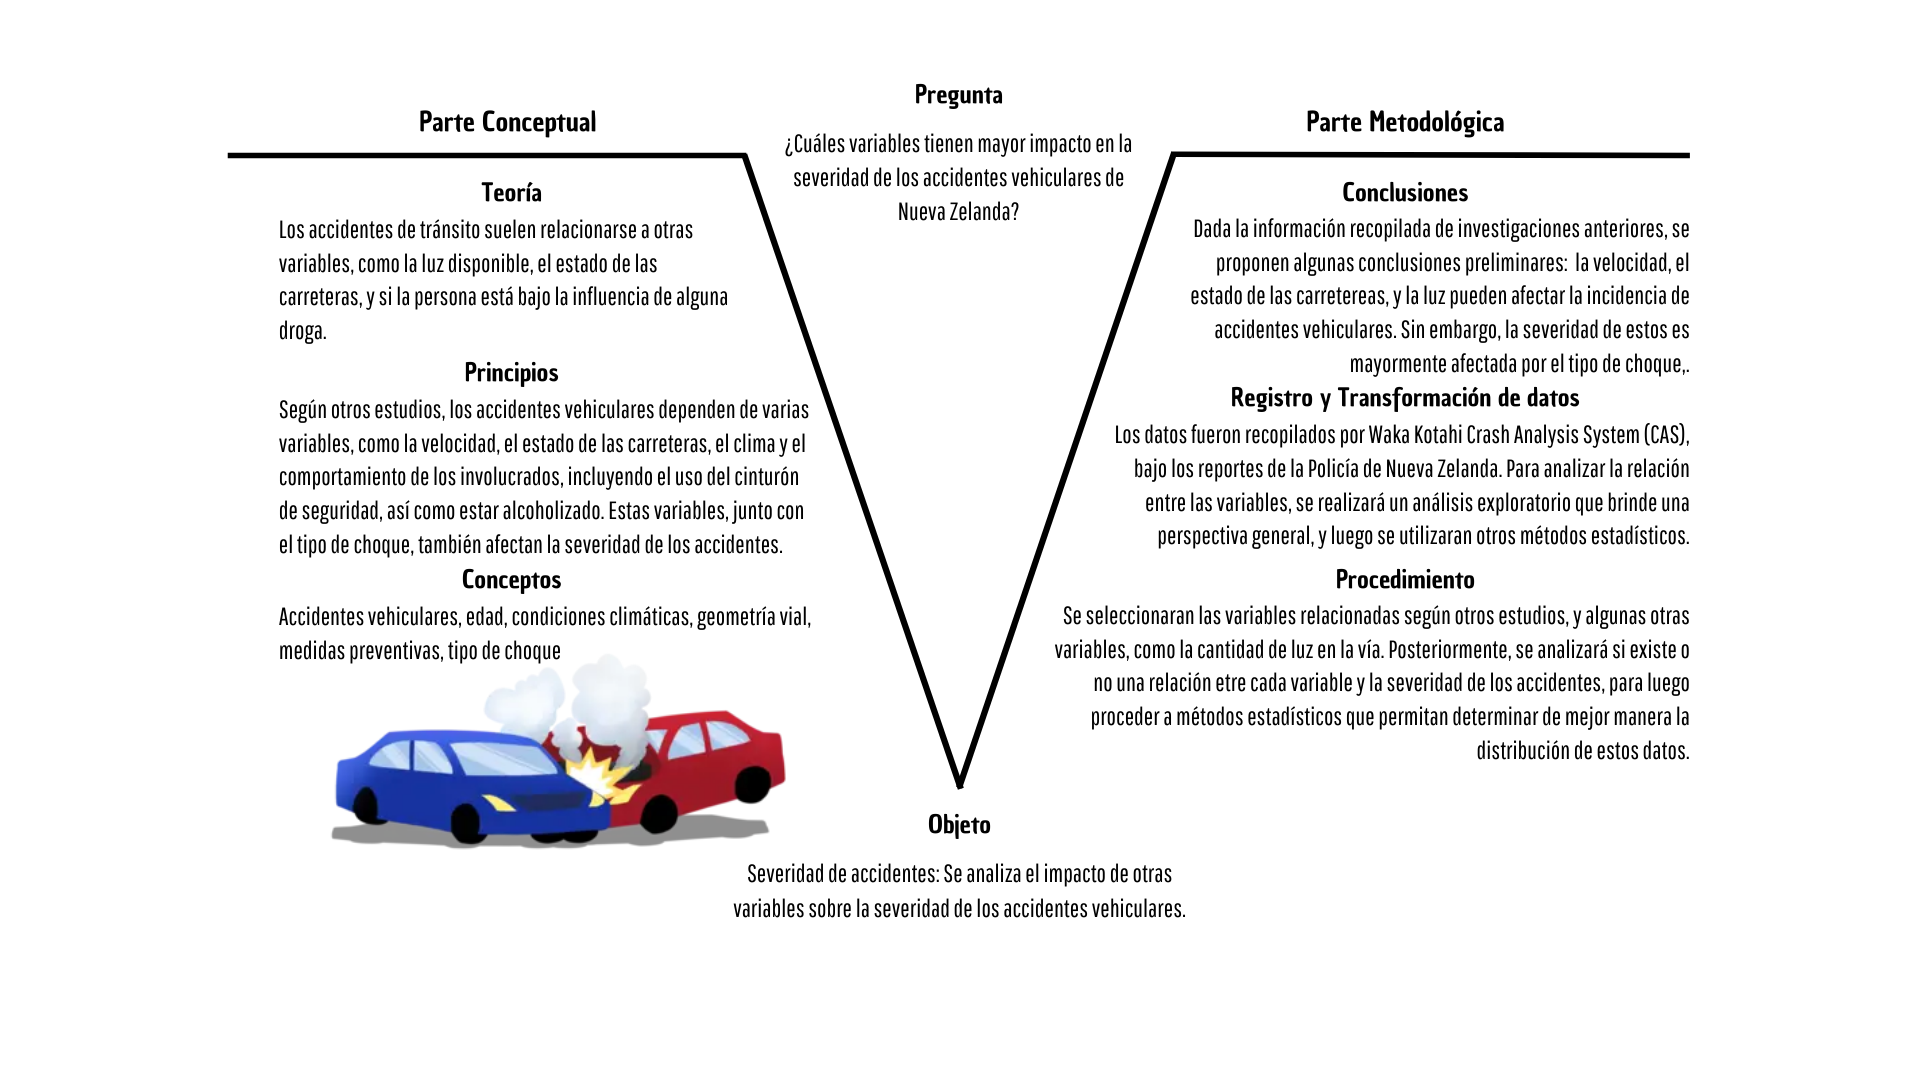
\includegraphics[width=1\linewidth]{V_Gowin_b2.png}
\caption{\label{fig:Gowin}V de Gowin}
\end{figure}

\section{Parte de escritura}

Los accidentes de tráfico representan una de las principales causas de muertes y lesiones en todo el mundo. En el caso de Nueva Zelanda, la seguridad vial ha sido una preocupación constante, y se ha buscado implementar diversas estrategias para reducir la siniestralidad en las carreteras. Sin embargo, para mejorar la efectividad de estas estrategias, es fundamental tratar de identificar cuáles son las variables que poseen una mayor influencia o impacto en la severidad de los accidentes. Por ello, este trabajo busca responder a la pregunta: ¿Cuáles variables tienen mayor impacto en la severidad de los accidentes de tráfico en Nueva Zelanda?

De acuerdo con \cite{BuitragoRamírezFrancisco2019Vpdv}, entre los diversos factores que podrían influir en la severidad de un accidente de tránsito están los factores humanos, vehiculares, ambientales y de infraestructura. Entre ellos, más específicamente, se encuentran la atención, concentración y condición psíquico-física del conductor, las características de los vehículos, los objetos y la carga transportada, las condiciones meteorológicas, el ámbito urbano o interurbano en el que ocurre el accidente y el estado de las carreteras.

Asimismo, en busca de garantizar la calidad y veracidad del análisis, este trabajo utilizará como fuente principal los datos provenientes de la Agencia de Transporte Waka Kotahi de Nueva Zelanda. De esta forma, como el objetivo es determinar las variables con mayor impacto o incidencia en la severidad de los accidentes de tráfico mediante el uso de métodos estadísticos rigurosos, se pretende establecer si existe una relación significativa entre las variables analizadas y la severidad de los accidentes.

Para ello, se plantean las variables de interés, es decir, las que podrían tener un impacto significativo en la severidad de los accidentes, tomando en cuenta que la base de datos cuenta con 72 variables distintas:

\begin{itemize}
\item Velocidad recomendada
\item Recuento de víctimas fatales
\item Período de vacaciones
\item Iluminación
\item Recuento de víctimas con lesiones menores
\item Peatón
\item Superficie de la carretera
\item Recuento de víctimas con lesiones graves
\item Límite de velocidad
\item Clima
\end{itemize}

A su vez, para determinar cuáles de estas variables tienen una relación estadísticamente significativa con la severidad del accidente, se emplearán los siguientes métodos de análisis de datos:

\begin{itemize}
\item \textbf{Prueba Chi-cuadrado}: Se utiliza para evaluar la independencia entre variables categóricas.
\item \textbf{Tablas de contingencia}: Permiten observar distribuciones conjuntas de variables y detectar patrones de asociación.
\item \textbf{Prueba t de Student}: Se usa cuando no conocemos ni la media ni la desviación estándar de nuestra población.
\item \textbf{P-value}: Sirve para determinar la significancia estadística de los resultados obtenidos en los análisis previos, estableciendo si la relación entre variables es lo suficientemente fuerte como para no ser atribuida al azar.
\end{itemize}

Además, el estudio tomará como referencia trabajos previos, como el de \cite{BuitragoRamírezFrancisco2019Vpdv}, que encontró que ciertos factores aumentan significativamente el riesgo de que una víctima resulte fallecida o termine en un estado crítico tras un accidente. Por ejemplo, determinó que los accidentes interurbanos incrementan en un 74.5\% el riesgo de fatalidad en comparación con los urbanos y que, en ciertas zonas de alta incidencia, este riesgo puede duplicarse o cuadruplicarse.

Por lo tanto, identificar las variables que tienen un mayor impacto en la severidad de los accidentes de tráfico permitirá la implementación de estrategias de prevención más efectivas. Esto contribuirá a optimizar la asignación de recursos para la reducción de accidentes, disminuyendo tanto el número de incidentes como la cantidad de personas heridas o fallecidas como consecuencia de los mismos. Además, los hallazgos de este estudio pueden servir como base para futuras investigaciones en seguridad vial y políticas públicas.

\chapter*{Bitácora 2}
\section{Ordenamiento de literatura}

\section{Enlaces de literatura}

\section{Análisis Estadísticos}
\subsection{Análisis Descriptivo}

\subsection{Propuesta Metodológica}
Se pretende identificar qué variables tienen mayor impacto en la severidad de los accidentes de tráfico en Nueva Zelanda. Para ello, se utilizarán métodos estadísticos como la prueba Chi-cuadrado para variables categóricas, la prueba t de Student para comparar medias en variables continuas según la severidad, así como el análisis de significancia mediante el p-value. 

A continuación se definen estas metodologías, de acuerdo con el libro Probability and Statistics \cite{degroot2012probability}.

\subsubsection{T de Student}
Sea $X_1, \ldots, X_n$ una muestra aleatoria de variables aleatorias de distribución normal con media $\mu$ y varianza $\sigma^2$, ambas desconocida. \\
Se sabe que $n^{1/2}(\overline{X}_n - \mu)/\sigma'$ tiene la distribución $t$ con $n - 1$ grados de libertad. Sea $T_{n-1}^{-1}$ la función cuantil de la distribución $t$ con $n - 1$ grados de libertad.\\
Entonces, para probar $H_0: \mu < \mu_0$ versus $H_1: \mu > 0$ a un nivel $\alpha_0$, se rechaza $H_0$ si $n^{1/2}(\overline{X}n - \mu_0)/\sigma' > T_{n-1}^{-1}(1 - \alpha_0)$. \\
Para probar $H_0: \mu = \mu_0$ versus $H_1: \mu \neq \mu_0$, se rechaza $H_0$ si $|n^{1/2}(\overline{X}n - \mu_0)/\sigma'| \geq T{n-1}^{-1}(1 - \alpha_0/2)$. \\
Las funciones de potencia de cada una de estas pruebas pueden ser escritas en términos de la función de distribución acumulativa de una distribución $t$ no central con $n - 1$ grados de libertad y parámetro de no centralidad $\psi = n^{1/2}(\mu - \mu_0)/\sigma$.

\subsubsection{Valor p}
El valor p, o nivel observao de significancia, es el nivel más pequeño $\alpha_0$ tal que rechazaríamos la hipótesis nula al nivel $\alpha_0$ con los datos observados. Es decir, si un experimentador rechaza una hipótesis nula si y solo si el valor $p$ es a lo sumo $\alpha_0$ está utilizando una prueba con nivel de significancia $\alpha_0$. De la misma manera, un experimentador que desea una prueba de nivel $\alpha_0$ rechazará la hipótesis nula si y solo si el valor $p$ es a lo sumo $\alpha_0$.

Para pruebas de la forma "rechazar la hipótesis nula cuando $T \geq c$" para un único estadístico de prueba $T$, hay una manera directa de calcular los valores $p$. 
Para cada $t$, sea $\delta_t$ la prueba que rechaza $H_0$ si $T \geq t$. Entonces el valor $p$ cuando se observa $T = t$ es el tamaño de la prueba $\delta_t$.
Es decir,
\begin{equation}
p = \sup_{\theta \in \Omega_0} \pi(\theta|\delta_t) = \sup_{\theta \in \Omega_0} \text{Pr}(T \geq t|\theta).
\end{equation}

Típicamente, $\pi(\theta|\delta_t)$ se maximiza en algún $\theta_0$ en la frontera entre $\Omega_0$ y $\Omega_1$.


\subsubsection{Prueba Chi-cuadrado}
Para llevar a cabo una prueba $\chi^2$ de bondad de ajuste de las hipótesis, el estadístico $Q$ definido por 
$$Q = \sum_{i=1}^{k} \frac{(N_i - np_i^0)^2}{np_i^0}$$
debe ser modificado porque el número esperado $np_i^0$ de observaciones de tipo $i$ en una muestra aleatoria de $n$ observaciones ya no está completamente especificado por la hipótesis nula $H_0$. The modification that se uses consiste simplemente in reemplazar $np_i^0$ por el EMV of this nmero esperado bajo la suposición of that $H_0$ es verdadera.\\
En otras palabras, si $\hat{\theta}$ denota el E.M.V. del vector de parámetros $\theta$ basado en los números observados $N_1, \ldots, N_k$, entonces el estadístico $Q$ se define como sigue:

\begin{align} \label{Q_chi_test}
Q = \sum_{i=1}^{k} \frac{[N_i - n\pi_i(\hat{\theta})]^2}{n\pi_i(\hat{\theta})}.
\end{align}

Nuevamente, es razonable basar una prueba de las hipótesis de la forma
\begin{align} \label{pruebaH}
H_0: \quad &\text{Existe un valor de } \theta \in \Omega \text{ tal que}\\
&p_i = \pi_i(\theta) \text{ para } i = 1, \ldots, k.\\
H_1: \quad &\text{La hipótesis } H_0 \text{ no es verdadera.}
\end{align}
en este estadístico $Q$ rechazando $H_0$ si $Q \geq c$, donde $c$ es una constante apropiada. 

En 1924, R. A. Fisher demostró el siguiente resultado,

\paragraph{Prueba $\chi^2$ para Hipótesis Nula Compuesta}

Supongamos que la hipótesis nula $H_0$ en \ref{pruebaH} es verdadera y que se satisfacen ciertas condiciones de regularidad. Entonces, cuando el tamaño de la muestra $n \to \infty$, la f.d.a. de $Q$ en \ref{Q_chi_test} converge a la f.d.a. de la distribución $\chi^2$ con $k - 1 - s$ grados de libertad.

Cuando el tamaño de la muestra $n$ es grande y la hipótesis nula $H_0$ es verdadera, la distribución de $Q$ será aproximadamente una distribución $\chi^2$. Para determinar el número de grados de libertad, debemos restar $s$ del número $k - 1$, porque ahora estamos estimando los $s$ parámetros $\theta_1, \ldots, \theta_s$ cuando comparamos el número observado $N_i$ con el número esperado $n\pi_i(\hat{\theta})$ para $i = 1, \ldots, k$. \\ 
Para que este resultado sea válido, es necesario satisfacer las siguientes condiciones de regularidad: Primero, el E.M.V. $\hat{\theta}$ del vector $\theta$ debe ocurrir en un punto donde las derivadas parciales de la función de verosimilitud con respecto a cada uno de los parámetros $\theta_1, \ldots, \theta_s$ sean iguales a 0.

\subsubsection{Tablas de Contingencia}
Una tabla de contingencia es una tabla en la que cada observación se clasifica de al menos dos maneras.
Una tabla de contingencias es bidireccional si solo se consideran dos clasificaciones para cada entrada.

En general, se considera una tabla de contingencia bidireccional que contiene $R$ filas y $C$ columnas. Para $i = 1, \ldots, R$ y $j = 1, \ldots, C$, denotaremos $p_{ij}$ como la probabilidad de que un individuo seleccionado al azar de una población dada sea clasificado en la $i$-ésima fila y la $j$-ésima columna de la tabla. Además, denotaremos $p_{i+}$ como la probabilidad marginal de que el individuo será clasificado en la $i$-ésima fila de la tabla y $p_{+j}$ denotará la probabilidad marginal de que el individuo será clasificado en la $j$-ésima columna de la tabla. Así,

\begin{align}
p_{i+} = \sum_{j=1}^{C} p_{ij} \quad \text{y} \quad p_{+j} = \sum_{i=1}^{R} p_{ij}.
\end{align}

Además, dado que la suma de las probabilidades para todas las celdas de la tabla debe ser 1, entonces

\begin{align}
\sum_{i=1}^{R} \sum_{j=1}^{C} p_{ij} = \sum_{i=1}^{R} p_{i+} = \sum_{j=1}^{C} p_{+j} = 1.
\end{align}

Al tomar una muestra aleatoria de $n$ individuos de la población dada. Para $i = 1, \ldots, R$, y $j = 1, \ldots, C$, denotaremos $N_{ij}$ como el número de individuos que están clasificados en la $i$-ésima fila y la $j$-ésima columna de la tabla. Además, se denotará $N_{i+}$ como el número total de individuos clasificados en la $i$-ésima fila y $N_{+j}$ denotará el número total de individuos clasificados en la $j$-ésima columna.

Así,

\begin{align}
N_{i+} = \sum_{j=1}^{C} N_{ij} \quad \text{y} \quad N_{+j} = \sum_{i=1}^{R} N_{ij}.
\end{align}

También,

\begin{align}
\sum_{i=1}^{R} \sum_{j=1}^{C} N_{ij} = \sum_{i=1}^{R} N_{i+} = \sum_{j=1}^{C} N_{+j} = n.
\end{align}

Sobre la base de estas observaciones, se deben probar las siguientes hipótesis:
\begin{align}
H_0&: \quad p_{ij} = p_{i+}p_{+j} \quad \text{para} \; i = 1, \ldots, R \; \text{y} \; j = 1, \ldots, C, \\
H_1&: \quad \text{La hipótesis } H_0 \text{ no es verdadera.}
\end{align}

\paragraph*{La Prueba $\chi^2$ de Independencia}
Para aplicar la prueba $\chi^2$, cada individuo en la población de la cual se toma la muestra debe pertenecer a una de las $RC$ celdas de la tabla de contingencia. Bajo la hipótesis nula $H_0$, las probabilidades desconocidas $p_{ij}$ de estas celdas se han expresado como funciones de los parámetros desconocidos $p_{i+}$ y $p_{+j}$. Dado que $\sum_{i=1}^{R} p_{i+} = 1$ y $\sum_{j=1}^{C} p_{+j} = 1$, el número real de parámetros desconocidos a estimar cuando $H_0$ es verdadera es $s = (R - 1) + (C - 1)$, o $s = R + C - 2$.

Para $i = 1, \ldots, R$, y $j = 1, \ldots, C$, denote $\hat{E}_{ij}$ el E.M.V., cuando $H_0$ es verdadera, del número esperado de observaciones que serán clasificadas en la $i$-ésima fila y la $j$-ésima columna de la tabla, entonces

\begin{align}
Q = \sum_{i=1}^{R} \sum_{j=1}^{C} \frac{(N_{ij} - \hat{E}_{ij})^2}{\hat{E}_{ij}}.
\end{align}

Además, dado que la tabla de contingencia contiene $RC$ celdas, y dado que $s = R + C - 2$ parámetros deben ser estimados cuando $H_0$ es verdadera, se deduce que cuando $H_0$ es verdadera y $n \to \infty$, la función de distribución acumulada (f.d.a.) de $Q$ converge a la f.d.a. de la distribución $\chi^2$ para la cual el número de grados de libertad es $RC - 1 - s = (R - 1)(C - 1)$.

A continuación, consideraremos la forma del estimador $\hat{E}_{ij}$. El número esperado de observaciones en la $i$-ésima fila y la $j$-ésima columna es simplemente $np_{ij}$. Cuando $H_0$ es verdadera, $p_{ij} = p_{i+}p_{+j}$. Por lo tanto, si $\hat{p}_{i+}$ y $\hat{p}_{+j}$ denotan los E.M.V. de $p_{i+}$ y $p_{+j}$, entonces se deduce que $\hat{E}_{ij} = n\hat{p}_{i+}\hat{p}_{+j}$. Además, como $p_{i+}$ es la probabilidad de que una observación sea clasificada en la $i$-ésima fila, $\hat{p}_{i+}$ es simplemente la proporción de observaciones en la muestra que están clasificadas en la $i$-ésima fila; es decir, $\hat{p}_{i+} = N_{i+}/n$. De manera similar, $\hat{p}_{+j} = N_{+j}/n$, y se deduce que

\begin{align}
\hat{E}_{ij} = n\left(\frac{N_{i+}}{n}\right)\left(\frac{N_{+j}}{n}\right) = \frac{N_{i+}N_{+j}}{n}.
\end{align}

Al sustituir este valor de $\hat{E}_{ij}$, se puede calcular el valor de $Q$ a partir de los valores observados de $N_{ij}$. La hipótesis nula $H_0$ debe ser rechazada si $Q > c$, donde $c$ es una constante apropiadamente elegida. Cuando $H_0$ es verdadera, y el tamaño de la muestra $n$ es grande, la distribución de $Q$ será aproximadamente la distribución $\chi^2$ con $(R - 1)(C - 1)$ grados de libertad.

\subsection{Fichas de Resultados}


\bibliographystyle{apalike}
\bibliography{referencias}
\nocite{*}

\end{document}
